\documentclass[12pt]{article}
\usepackage[margin = 1in]{geometry}
\usepackage{makeidx}
\usepackage{amsmath,amsfonts,amssymb,amsthm}
\usepackage{graphics}
\usepackage{graphicx}
\allowdisplaybreaks
\thispagestyle{empty}
\usepackage{framed}

\usepackage{subfigure}

\usepackage{framed}
\usepackage{mathrsfs}
\usepackage{enumerate}
\usepackage{tikz}
\usetikzlibrary{matrix}
\usepackage[all]{xy}
\usetikzlibrary{shapes}
\usetikzlibrary{decorations.markings}
\usepackage{hyperref}
\usepackage{multirow}
\usepackage{bm}

\usepackage[T1]{fontenc}

% Tim's Commands
\newcommand{\cA}{\mathcal A}
\newcommand{\cB}{\mathcal B}
\newcommand{\cC}{\mathcal C}
\newcommand{\cD}{\mathcal D}
\newcommand{\cE}{\mathcal E}
\newcommand{\cP}{\mathcal P}
\newcommand{\cS}{\mathcal S}
\newcommand{\cT}{\mathcal T}
\newcommand{\cL}{\mathcal L}
\newcommand{\K}{\mathbb K}
\newcommand{\N}{\mathbb N}
\newcommand{\Z}{\mathbb Z}
\newcommand{\R}{\mathbb R}
\newcommand{\Q}{\mathbb Q}

%\newcommand{\max}{\operatornamewithlimits{\mbox{argmax}\,}}

\newcommand{\Aff}{\mathrm{Aff}\,}
\newcommand{\Abb}{{\textrm Abb}}

\newcommand{\adj}{{\textrm adj}\;}
\newcommand{\aff}{\mathrm{aff}\,}
\newcommand{\Def}{\mathrm{def}\;}
\newcommand{\End}{\mathrm{End}}

\newcommand{\Aut}{\mathrm{Aut}}
\newcommand{\GL}{\text{GL}}

\newcommand{\Hom}{\textrm Hom}





\newcommand{\bS}{\mathbb{S}}
\newcommand{\Sn}{\bS^n}




\newcommand{\bE}{\mathbb E}

\newcommand{\cN}{\mathcal N}

\newcommand{\B}{\mathbb B}
\newcommand{\bB}{\mathbb B}
%\newcommand{\C}{\mathbb C}

\newtheorem{proposition}{Proposition}[section]
\newtheorem{theorem}{Theorem}[section]
\newtheorem{lemma}{Lemma}[section]

\def\argmin{ \mathrm{argmin}}

\def\argmax{ \mathrm{argmax}}

\newcommand{\bd}{\mathrm{bd}\,}
\newcommand{\bi}{\binom}
\newcommand{\Char}{\mathrm{char}}
\newcommand{\cone}{\mathrm{cone}\;}
\newcommand{\co}{\mathrm{conv}\,}
\newcommand{\core}{\mathrm{core}\,}
\newcommand{\cl}{\mathrm{cl}\,}
\newcommand{\clco}{\overline{\mathrm{conv}}\,}
\newcommand{\diag}{\mathrm{diag}\,}
\newcommand{\dist}{\mathrm{dist}\,}
\newcommand{\dom}{\mathrm{dom}\,}
\newcommand{\conjug}{\;\overset{*}{\longleftrightarrow }\;}
\newcommand{\epi}{\mathrm{epi}\,}
\newcommand{\ext}{\mathrm{ext}\,}
\def\elim{{\textrm e-}\hspace{-0.5pt}\lim}
\def\glim{{\textrm g-}\hspace{-0.5pt}\lim}
\newcommand{\gph}{\mathrm{gph}\,}
\newcommand{\grad}{\mathrm{grad}\;}
\newcommand{\id}{\mathrm{id}\,}
\newcommand{\ip}[1]{\left\langle #1 \right\rangle}
\newcommand{\ind}{\mathrm{Ind}\,}
\newcommand{\inter}{\mathrm{int}\,}
\newcommand{\im}{\mathrm{rge}\,}
\newcommand{\Ima}{\mathrm{Im}}
\newcommand{\lev}{\mathrm{lev}}
\def\Lim{\mathop{{\textrm Lim}\,}}
\def\Liminf{\mathop{{\textrm Lim}\,{\textrm inf}}}
\def\Limsup{\mathop{{\textrm Lim}\,{\textrm sup}}}
\newcommand{\nul}{\mathrm{nul}\,}
\newcommand{\p}{\partial}
\newcommand{\rge}{\mathrm{rge}\,}

\newcommand{\rank}{\mathrm{rank}\,}

\newcommand{\Real}{\mathrm{Re}}
\newcommand{\sgn}{\mathrm{sgn}?}
\newcommand{\rbar}{\overline{\mathbb R}}
\newcommand{\rp}{\mathbb R\cup \{+\infty\}}
\newcommand{\rbd}{\mathrm{rbd}\,}
\newcommand{\ri}{\mathrm{ri}\,}
\newcommand{\set}[2]{\left\{#1\,\left\vert\; #2\right.\right\}}

\newcommand{\Uni}{\mathrm{U}}
\newcommand{\Orth}{\mathrm{O}}
\newcommand{\SU}{\mathrm{SU}}
\newcommand{\SO}{\mathrm{SO}}

\newcommand{\spn}{\mathrm{span}\,}

\newcommand{\Sym}{\mathrm{Sym}\,}

\newcommand{\tr}{\mathrm{tr}\,}

\newcommand{\lin}{\mathrm{span}\,}

\newcommand{\AND}{\quad\mbox{and}\quad}
\newcommand{\IFF}{\quad\Longleftrightarrow\quad}

% definition of Cartesian products
\def\XX{\operatornamewithlimits{\mbox{\sf\large X}}}
\def\XXX{\operatornamewithlimits{\mbox{\sf\Large X}}}

\include{macros}
\pagestyle{empty}

\usepackage[algoruled, linesnumbered, shortend, lined]{algorithm2e}
\usepackage{algpseudocode}

\begin{document}


\SetAlgoSkip{bigskip}
\SetKwInput{Input}{Input\hspace{34pt}{ }}
\SetKwInput{Output}{Output\hspace{27pt}{ }}
\SetKwInput{Initialize}{Initialize\hspace{20pt}{ }}
\SetKwInput{Parameters}{Parameters\hspace{2pt}{ }}

\newcommand{\prox}{\text{prox}}

\noindent
\parbox{5cm}
{\begin{center}
McGill University\\
Department of\\ Mathematics and Statistics \\
Courtney~Paquette
\end{center}}
\hfill
\parbox{4.3cm}{\center

\includegraphics[scale=0.3]{mcgill.pdf}}

\vspace{0.5cm}
\begin{center}

{\large \bfseries MATH 463/563 - Convex Optimization \\
\hfill\\
Project Description \\  }
Due Date: Tuesday, April 11 by 11:59 pm (local Montreal)\\
Submission Method: CrowdMark for the report and email with subject line \texttt{lastname firstname project code} and in the email, a list of all the group members names (first last and student numbers).  

\end{center}

\vspace{0.5cm}

\section{Project overview}

The project for this course involves the implementation of optimization algorithms for image de-blurring and de-noising. This document describes the algorithms that you are required to implement and further guidelines that you are to follow.  It also describes a set of problems that you are asked to solve and the expectations of a written report that you are asked to submit with your code.  A \LaTeX\ template (\texttt{project\_template.zip}) has been posted on myCourses for you to use to write your project report.

 Rather than submit each of these algorithms as separate pieces of code, you are asked to \emph{combine} all of these algorithms into a single software package.  You will also be required to implement more algorithms and options, allowing flexibility for users of your code.  All requirements are described in this document.

\subsection{Image De-blurring and De-noising} 
The image de-blurring problem is to recover the original sharp image using a mathematical model fo the blurring process. Many real-life optical systems that cause blurring can be approximated by linear models. Therefore, we use a linear model in our problem too. 

We assume that the blurred image is generated from the original image by a convolution with a spatially-invariant kernel (called \textit{point spread function} or \textit{PSF} in the image processing community). The kernel is typically much smaller in size than the image itself. In MATLAB, we use the function \texttt{fspecial} and \texttt{conv2} for the convolutions. The explicit blurring model we consider is 
\[k * x + \eta = b\]
where $*$ represents the 2D-convolution operator, $b$ the corrupted image, $k$ a non-negative blue kernel with relatively small support, $x$ the original \textit{black and white} image (converted to a matrix with values representing the amount of black color per pixel and \textit{resized so that each pixel is between 0 and 1}), and $\eta$ additive noise. Three different kernels and the corresponding blurred images are shown in Figure~\ref{tb: Examples}.

\begin{center}
\begin{figure}[h!]
\advance\leftskip-1cm
\vspace{-0.2in}
\begin{tabular}{ccc}
\begin{subfigure}[Gaussian Blur with Kernel]{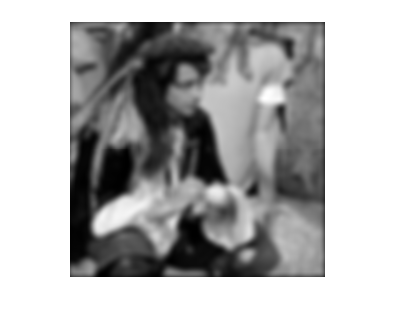
\includegraphics[trim
    = 0mm 0mm 0mm 0mm, clip, width=5cm]{ImagesIntro/gaussian_blur_pic.png}} \end{subfigure}  & 
\begin{subfigure}[No Blur with Identity Kernel]{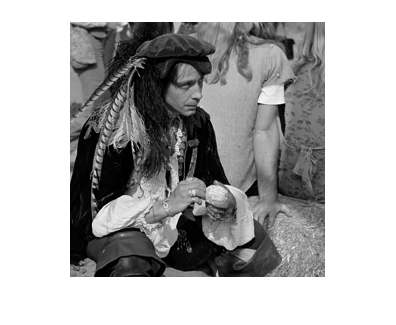
\includegraphics[
  width=5cm]{ImagesIntro/True_Image.png}} 
\end{subfigure}  &
\begin{subfigure}[Motion Blur with Kernel]{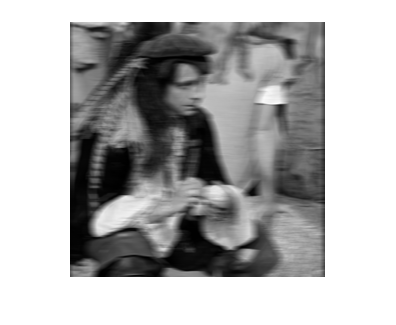
\includegraphics[trim = 0mm 0mm 0mm 0mm, clip,
  width=5cm]{ImagesIntro/motion_blur_pic.png}} \end{subfigure} \\
\begin{subfigure}{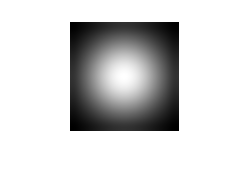
\includegraphics[trim = 0mm 0mm 0mm 0mm, clip,
  width=5cm]{ImagesIntro/gaussian_blur.png}} \end{subfigure}  & 
\begin{subfigure}{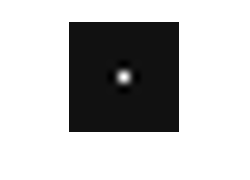
\includegraphics[trim = 0mm 0mm 0mm 0mm, clip,
  width=5cm]{ImagesIntro/identity_blur.png}} \end{subfigure}  &
\begin{subfigure}{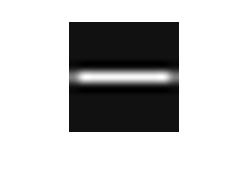
\includegraphics[trim = 0mm 0mm 0mm 0mm, clip,
  width=5cm]{ImagesIntro/motion_blur.png}} \end{subfigure} \\
\end{tabular}
\caption{Examples of Different Blur Kernels applied to the Man with
  the Hat Picture} \label{tb: Examples}
\end{figure}
\end{center}

Since convolution is a linear transformation, it can be represented as a matrix multiplication. The matrix representation of convolution, $K$, is determined from the PSF and the boundary conditions, which describe our assumptions of the scene just outside our image. Modeling the right boundary conditions is critical because different conditions lead to different matrix structures, and so one cannot use the same factorization tricks in all cases. In our case, we assume periodic boundary conditions, that is, the image repeats endlessly in every direction, like tiles on a floor. This prevents boundary artifacts in the blurred image (so the recovered image is also free from boundary artifacts). Another good option would be using zero-padding, but it would work well only if the image had mostly dark pixels near the boundary (like in astronomical images). 

With our assumptions, the blurring matrix $K$ turns out to be block circulant with circulant blocks (BCCB). A circulant matrix is diagonalized by the Discrete Fourier Transform (DFT) matrix of the same size, with eigenvalues being the DFT of the first row of the matrix (note that the first row of a circulant matrix gives us all the information about the matrix, so it is not surprising that the eigenvalues of the matrix can be derived from the first row alone). This property is derived directly by writing out the Circular Convolution Theorem in matrix form. This property can be extended to BCCB matrices to show that they have a spectral decomposition $K = Q^{H}\text{diag}(\lambda)Q$ where $Q = W\otimes W$ is the Kronecker product of the the length-$N$ DFT matrix with itself, and $\lambda$ is the $2D$ DFT of the convolution kernel.

This structure can be exploited nicely in our problem, which is a specific case of the generic convex optimization problem 
\[ \min_{x} \phi_f(Kx-b) + \phi_r(x) + \phi_s(\cdot). \]
with $K$ representing the blurring matrix, $\phi_f(\cdot)$ ensuring
fidelity of the recovered image, and $\phi_r(\cdot)$ and $\phi_S(\cdot)$ imposing certain properties on the recovered image. Usually,
solving this minimization problem requires solving a system of linear
equations with coefficients $I + K^{T}K$. The size of the matrix $K$ is extremely big, thus making it impractical to try and solve for this system of equations directly. But by the property of BCCB matrices mentioned in the previous paragraph and using the FFT algorithm to calculate the DFT (MATLAB function \texttt{fft2}), we can solve this system of equations in $\mathcal{O}(N^2\log(N))$ operations.

With this set-up, we tackle the non-blind deconvolution problem. 


\subsubsection{Non-Blind Framework}
In the non-blind formulation of the problem, we assume that the kernel
is known (for example, a Gaussian or linear kernel as in Figure
(\ref{tb: Examples}) ) and attempt to recover the true image from a
blurred, noisy observation. We formulate the image deblurring as the optimization problem
\[ \text{minimize}_x \quad \phi_f (Kx-b) + \phi_r(x) + \phi_s(Dx), \]
where  $\phi_f, \phi_r, \phi_s$ are convex penalty or indicator functions, $K$ is the blurring operator, $b$ is the blurred image, and $D$ is the discrete gradient operator
\[ D = \left[ \begin{array}{c} I \otimes \tilde{D} \\ \tilde{D} \otimes I \end{array}\right], \quad
\tilde{D} = \left[ \begin{array}{cccccc} 
-1 & 1 & 0 & \ldots & 0 & 0 \\ 
0 &-1 & 1 & \ldots & 0 & 0 \\ 
0 & 0 &-1 & \ldots & 0 & 0 \\ 
0 & 0 & 0 & \ldots & -1 & 1\\ 
1 & 0 & 0 & \ldots & 0 & -1 \\
\end{array}\right] \in \R^{N \times N} \]
as in \cite{Vandenberghe14}. The first $n$ rows of $D$ are the horizontal discretized derivative operator and the last $n$ rows are the vertical discretized derivative operator, so that minimizing $\phi_s(Dx)$ corresponds to ``smoothing" sharp edges in an image and getting rid of noise. Here $x,b\in \R^n$ are vectorized images, and $n= N^2$ is the number of pixels of the image. 

We will consider two particular formulations of this problem in this paper. The first, which is valid for any image we wish to deblur, is    
\begin{align}
\underset{x}{\text{minimize}} \quad \| Kx-b \|_1 + \delta_S(x) + \gamma \|Dx \|_{\text{iso}},  \label{eq: improblem1} 
\end{align}
where $S = \{ x: 0 \le x \le {\bf 1} \}$ is the range of allowed pixel
intensities (each image's intensity is normalized to lie within $0$
and $1$), $\gamma >0$, and 
\[ \| (x,y) \|_{\text{iso}} = \sum_{k=1}^n (x_k^2 + y_k^2)^{1/2}, \]
so that $\gamma \|Dx\|_{\text{iso}} = \gamma \| x\|_{TV}$ gives the total variation norm typically used in the literature. \textbf{Here we view $x$, the image, as a big vector; however when you implement this, you should implement it with $x$ as a matrix.} We choose an $l_1$ penalty on the residual $Kx-b$ to enforce sparsity because we would like the reconstructed image to be as exact as possible.

The other formulation will be 
\begin{align}
\underset{x}{\text{minimize}} \quad \| Kx-b \|^2_2 + \delta_S(x) + \gamma \|Dx \|_{\text{iso}}. 
\label{eq: improblem2} 
\end{align}

Here: If $x \in \mathbb{R}^n$, then $x \mapsto Dx =\begin{pmatrix} w_1 \\ w_2 \end{pmatrix}$ where $w_1, w_2 \in \mathbb{R}^n$. Then $\|Dx\|_{\text{iso}} = \|(w_1, w_2)\|_{\text{iso}}$. 

\subsection{Algorithms}

The algorithms we use to solve the non-blind image deblurring problem work for general
convex optimization problems of the form:
\begin{align}
\underset{x,y}{\min} \quad & f(x) + g(y) \label{eq: problem} \\
\text{subject to} \quad & Ax = y, \nonumber
\end{align}
where both $f$ and $g$ are closed, convex functions with inexpensive
prox-operators. Notice that both the problems we consider can be
written in this form, with 
\begin{gather*}
f(x) = \delta_S(x)\\
g \left( [ y_1 \; y_2  ]^T \right) = \| y_1 - b \|_1 + \gamma
\|(y_2, y_3)\|_{\text{iso}}, \quad A = \left[ \begin{array}{c} K \\
                                         D \end{array} \right], \text{ for Equation (\ref{eq:
  improblem1})},\\
\text{and} \quad g \left( [ y_1 \; y_2 ]^T \right) = \| y_1 - b \|_2^2 + \gamma
\|y_2\|_{\text{iso}}, \quad A = \left[ \begin{array}{c} K \\
                                         D \end{array} \right],  \text{ for Equation (\ref{eq:
  improblem2}).}
\end{gather*}

For the moment disregard (\ref{eq: problem}) and consider the problem
of finding an $x$ such that 
\begin{equation}
0 \in \mathcal{F}(x). \label{eq: monotone}
\end{equation}
Think of $\mathcal{F}$ as $\partial (f + g \circ A)(x)$ so you are trying to find a minimum (in fact, $\mathcal{F}$ is called a maximal
monotone operator). We will phrase (\ref{eq: problem}) in terms of different $\mathcal{F}$. The roots of $\mathcal{F}$
precisely coincide with fixed points of the resolvent. Therefore,
algorithms to solve for the roots often rely on the fixed point iteration scheme:
\[ x^k = (I + t\mathcal{F})^{-1}(x^{k-1}), \quad k = 1, 2, \hdots.\] 
This fixed point iteration is only useful in practice when the evaluation of the
resolvent is computationally easy. For many scenarios (including image
deblurring), this is not the case. Instead, a \textit{splitting
  algorithm} decomposes the monotone operator as $\mathcal{F} =
\mathcal{A} + \mathcal{B}$ where $\mathcal{A}, \mathcal{B}$ are
themselves maximal monotone operators whose resolvents are easy to
compute. 

As described in \cite{Eckstein92} and \cite{Vandenberghe14}, a simple
algorithm for solving $0 \in \mathcal{A} + \mathcal{B}$ is the
Douglas-Rachford iteration:
\begin{align}
x^k &= (I+t\mathcal{A})^{-1}(z^{k-1}) \label{eq: scheme1} \\
y^k &=(I + t \mathcal{B})^{-1}(2x^k - z^{k-1})\\
z^k &= z^{k-1} + \rho(y^k - x^k) \label{eq: scheme3}
\end{align}
where $t$ is a positive step size and $\rho \in (0, 2)$ is a
relaxation parameter. A derivation of the algorithm
described above is obtained by solving for the fixed points of $z^k = F(z^{k-1})$ where 
\[F(z) = z + (I + t\mathcal{B})^{-1} ( 2 (I+t \mathcal{A})^{-1}(z) -z)
- (I + t \mathcal{A})^{-1}(z).\]
Proven in \cite{Eckstein92}, the sequence $z^k$ converges to a limit of the
form $x + tv$ where $0 \in \mathcal{A}(x) + \mathcal{B}(x)$ and $v \in
\mathcal{A}(x) \cap \mathcal{-B}(x)$. For more information regarding
monotone operators see \cite{Rockafellar98}. 

Returning to the problem in (\ref{eq: problem}), optimality conditions
are stated in terms of a $0$ lying in some
subdifferential. For instance, one optimality condition is $0
\in \partial (f + g \circ A)(x) = \mathcal{F}(x)$. It is well known that subdifferentials of closed,
convex functions are maximal monotone operators. Therefore, optimizing
(\ref{eq: problem}) is analogous to finding a zero of the maximal
monotone operator which in turn is the
same as finding a fixed point of the resolvent. An example of a
monotone operator and its resolvent is the subdifferential and its
prox-operator. Unfortunately, the full prox-operator in the image
deblurring problem is expensive and so we
consider splitting algorithms. Natural choices to ``split'' the operator
$\mathcal{F}(x)$ into $\mathcal{A}(x) +
\mathcal{B}(x)$ are the subdifferentials of $f$ and $g$
and/or the subdifferentials of their conjugate duals. 
% Some important functions and
% their prox-operators to keep in mind throughout the paper are
% {\small \begin{align}
% f(x) = \norm{x}_1 \qquad & \prox_{tf}(x)_k = \text{sign}(x_k)
%                            \cdot \max \{ |x_k|-t, 0\}\\
% f((x,y)) = \norm{(x,y)}_{\text{iso}} 
%   \qquad & \prox_{tf}(x_k, y_k) \nonumber \\
% &  =  \begin{cases}
% \left (1- \frac{t}{(x_k^2+y_k^2)^{1/2}} \right ) \cdot (x_k, y_k) &
% \text{if } (x_k^2+y_k^2)^{1/2} >  t \\
% 0 & \text{otherwise}
% \end{cases}\\
% f(x) = \frac{1}{2} \norm{x}_2^2 \qquad & \prox_{tf}(x) =
%                                          \frac{x}{1+t} \\
% \text{$S$ closed convex, } f(x) = \delta_S(x) \qquad & \prox_{tf}(x)
% =\text{projection of $x$ onto $S$}\\
% f(x) = g(x+b) \qquad & \prox_{tf}(x) = \prox_{tg}(x+b)-b\\
% f^*(x) \qquad & \prox_{tf^*}(x) =  x-t \prox_{t^{-1} f}(x/t)\\
%                 & \text{(Moreau decomposition)} \nonumber
% \end{align}}
Another useful monotone
operator is the linear operator $\mathcal{F}(x) = Ax$ where $A$ is
skew-symmetric. As the notation suggests, the matrix inverse $(I +
\lambda A)^{-1}$ is its resolvent and is explicitly given by 
\begin{equation}
\begin{bmatrix}
I & \lambda C^T\\
-\lambda C & I
\end{bmatrix}^{-1} = \begin{bmatrix}
0 & 0\\
0 & I
\end{bmatrix} + \begin{bmatrix}
I\\
\lambda C
\end{bmatrix} (I + \lambda^2 C^TC)^{-1} \begin{bmatrix}
I\\
-\lambda C
\end{bmatrix}^T \label{eq: matrix resolvant}
\end{equation} 

In the next few sub-sections, we discuss four different algorithms to
solving (\ref{eq: problem}). The first three- Primal Douglas-Rachford,
Primal Dual Douglas-Rachford, and ADMM- use the iteration scheme
outlined in (\ref{eq: scheme1})-(\ref{eq: scheme3}) under different
optimality conditions (maximal monotone operators) and splittings. The
last algorithm, Chambolle Pock, approaches the problem from a
different perspective. We conclude the
introduction with a brief outline of the mathematics behind solving
the blind deconvolution problem. 

\subsubsection{Primal Douglas-Rachford Splitting (Spingarn's
  Method)} \label{sssec: DRprimal}
We can rewrite (\ref{eq: problem}) as:
\[ \min_{x,y} f(x)+g(y) + \delta_0 \big ( \begin{bmatrix} A & -I \\ \end{bmatrix} \begin{pmatrix} x\\ y \end{pmatrix} \big ).\]
The optimality condition for this \textit{primal problem} states that 
\[0 \in \partial f(x) + \partial
g(y) + \partial \delta_0 \big ( \begin{bmatrix} A & -I
  \\ \end{bmatrix} \begin{pmatrix} x\\ y \end{pmatrix} \big
) =: \mathcal{F}(x,y).\]
 Let $\mathcal{A}(x,y)
= \partial f(x) + \partial g(y)$ and $\mathcal{B}(x,y) = \partial \delta_0 \big ( \begin{bmatrix} A & -I
  \\ \end{bmatrix} (x,y)^T \big
)$ so that $\mathcal{F}(x,y) = \mathcal{A}(x,y) +
\mathcal{B}(x,y)$. Due to the separability of the variables, the
resolvent of $\mathcal{A}$ is $( \prox_{tf}(x), \prox_{tg}(y) )$, which
we assume is inexpensive to compute. Using the results in the previous
section, the operator $\mathcal{B}$'s resolvent is the projection $(x,y)$
of a vector $(\bar{x}, \bar{y})$ onto the subspace $\{(x,y) \, : \, Ax
= y\}$, expressed simply as
\[x = (I+A^TA)^{-1} (\bar{x} + A^T \bar{y}), \quad y = Ax.\]
Although there is a closed form, the inverse leads to implementation
difficulties as the size of $A$ is large in the problem we are considering. Applying the iteration
scheme (\ref{eq: scheme1})-(\ref{eq: scheme3}), the primal Douglas-Rachford Splitting
algorithm is stated below (Algorithm \ref{alg: DRprimal}).

\begin{algorithm}[h!]
 \SetKw{Null}{NULL}
 \SetKw{Return}{return}
 \Input{ Blurred image $b$, step size $t$, relaxation parameter $\rho$}
 \Output{ Deblurred image $x$ }
\Initialize{ $(z^0_1, z^0_2)$ }

\For { $k = 1, 2, \hdots, $ } {
  $x^k \leftarrow \prox_{tf}(z^{k-1}_1)$ \tcp*{Performs resolvent of $\mathcal{A}$} 
  $y^k \leftarrow \prox_{tg}(z^{k-1}_2)$ \;
  $u^k \leftarrow (I+A^TA)^{-1} \big ( 2x^k-z^{k-1}_1 +
  A^T(2y^k-z^{k-1}_2) \big )$ \tcp*{Performs
    resolvent of $\mathcal{B}$}
  $v^k \leftarrow A(u^k)$ \;
  $z^k_1 \leftarrow z^{k-1}_1 + \rho(u^k-x^k)$ \;
  $z^k_2 \leftarrow z^{k-1}_2 + \rho(v^k-y^k)$ \;
} 
\Return $x\text{Sol} = \prox_{tf}(z^k)$\;
\caption{Primal Douglas-Rachford Splitting}\label{alg: DRprimal} 
\end{algorithm}

\subsubsection{Primal-Dual Douglas Rachford Splitting} \label{sssec: DRpd}
Consider the dual problem of (\ref{eq: problem}):
\begin{equation}
\text{maximize}_y \quad -f^*(-A^Ty) - g^*(y) \label{eq: dual}
\end{equation}
The optimality conditions for both the primal (\ref{eq: problem}) and
the dual (\ref{eq: dual})  can be written as
\[ 0 \in \left[ \begin{array}{cccc} 0 & 0 & A^T & I \\ 0 & 0 & -I & 0 \\ -A & I & 0 & 0 \\ -I & 0 & 0 & 0 \end{array} \right] \left[ \begin{array}{c} x \\ y \\ z \\ w \end{array} \right] + \left[ \begin{array}{c} 0 \\ \partial g(y) \\ 0 \\ \partial f^* (w) \end{array} \right]
\]
where $w$ is the dual variable and $z$ is the dual multiplier for the constraint $y = Ax.$
This can be reduced to the smaller system
\[ 0 \in \left[ \begin{array}{cc} 0 & A^T \\ -A & 0 \end{array} \right] \left[ \begin{array}{c} x \\ z \end{array} \right] + \left[ \begin{array}{c}  \partial f(x) \\ \partial g^* (z) \end{array} \right],
\]
by using the relationships $\partial g^* = (\partial g)^{-1}$ and
$\partial f^* = (\partial f)^{-1}$ and eliminating variables. The right hand side is now a sum of two monotone operators in $x$ and $z$:
\[ \mathcal{A}(x,z) =  \left[ \begin{array}{c}  \partial f(x)
                                \\ \partial g^* (z) \end{array}
                            \right], \quad\mathcal{B}(x,z) =
                            \left[ \begin{array}{cc} 0 & A^T \\ -A &
                                                                     0 \end{array} \right] \left[ \begin{array}{c} x \\ z \end{array} \right], \]
which we will use as the ``split'' for the monotone operator. Unlike the ``split'' in the Primal Douglas-Rachford algorithm, this
uses both optimality conditions of the primal problem \textit{and} the
dual problem.  Applying the iteration
scheme (\ref{eq: scheme1}-\ref{eq: scheme3}), the primal Douglas-Rachford Splitting
algorithm is stated below (Algorithm \ref{alg: DRpd}).

\begin{algorithm}[h!]
 \SetKw{Null}{NULL}
 \SetKw{Return}{return}
 \Input{ Blurred image $b$, step size $t$, relaxation parameter $\rho$}
 \Output{ Deblurred image $x$ }
\Initialize{ $p^0, q^0$ }

\For { $k = 1, 2, \hdots, $ } {
  $x^k \leftarrow \prox_{tf}(p^{k-1}_1)$ \tcp*{Performs resolvent of $\mathcal{A}$} 
  $z^k \leftarrow \prox_{tg^*}(q^{k-1})$ \;
  $\begin{bmatrix} w^k\\ v^k  \end{bmatrix} = \begin{bmatrix} I &
   t A^T\\ -t A & I \end{bmatrix}^{-1} \begin{bmatrix}
    2x^k-p^{k-1}\\ 2z^k-p^{k-1} \end{bmatrix} $ \tcp*{Performs resolvent of $\mathcal{B}$} 
  $p^k \leftarrow p^{k-1} + \rho(w^k-x^k)$ \;
  $q^k \leftarrow q^{k-1} + \rho(v^k-z^k)$ \;
} 
\Return $x\text{Sol} = \prox_{tf}(p^k)$\;
\caption{Primal-Dual Douglas-Rachford Splitting}\label{alg: DRpd} 
\end{algorithm}

\subsubsection{ADMM (Dual Douglas-Rachford)}  \label{sssec: ADMM}
It can be shown that the alternating direction method of multipliers (ADMM) is exactly the Douglas-Rachford algorithm applied to the dual problem (\ref{eq: dual}), which we rewrite as
\begin{equation}
\text{minimize}_z \quad f^*(-A^Tz) + g^*(z)  := h(z) + k(z). \label{eq: dual2}
\end{equation}
The optimality conditions for (\ref{eq: dual2}) are precisely $0 \in \partial h(z) + \partial k(z).$ This is a sum of two maximal monotone operators $\mathcal{A}(z) = \partial h(z) $ and $\mathcal{B}(z) = \partial k(z)$, with resolvents $\prox_{th}(z)$ and $\prox_{tk}(z)$, respectively. An equivalent formulation of the Douglas-Rachford iteration for this problem, obtained by simply interchanging the order of the updates and performing a change of variables, is thus:
\begin{align}
v^k &= \prox_{th} (z^{k-1} - w^{k-1})\\
z^k &= \prox_{tk} (v^k + w^{k-1} ) \\
w^k &= w^{k-1}+ \rho v^k + (1-\rho)z^{k-1} - z^k.
\end{align}

\begin{proposition} If $h(z) = f^*(-A^Tz),$ then $\prox_{th}(z)$ can be computed by the following:
\[ \hat{x} = \underset{x}{\arg \min} \left( f(x) + z^T Ax + \frac{t}{2} \|Ax \|^2 \right) \]
\[ \prox_{th}(z) = z+ tA\hat{x}. \]
\end{proposition}

\begin{proof} 
Notice that $\hat{x}$ as given above is optimal for
\begin{align*}
 \text{minimize} \quad & f(x) + \frac{t}{2} \|w\|_2^2 \\
\text{subject to} \quad & w = Ax + z/t,
\end{align*}
where $z$ is fixed and $x,w$ are the variables. The optimality conditions for the above are $A\hat{x} + z/t = \hat{w},$ $-A^T\hat{u} \in \partial f(\hat{x}),$ and $t\hat{w}=\hat{u},$ where $u$ is the dual multiplier. Eliminating $x$ and $w$ and using the relationship $(\partial f)^{-1} = \partial f^*$, this is equivalent to the condition that $0 \in - A \partial f^*(-A^T \hat{u})+ \frac{1}{t}(\hat{u}-z) ,$ which is precisely the optimality condition that guarantees $\hat{u} = \prox_{th}(z) = \arg \min _u f^*(-A^Tu) + \frac{t}{2} \|u-z\|_2^2$. Combining these optimality conditions also leads to the relationship $\hat{u} = z+tA\hat{x},$ which proves the proposition.
\end{proof}

By this proposition (applied to both $h$ and $k$ in (\ref{eq: dual2})) the Douglas-Rachford algorithm on the dual can be rewritten as
\begin{align*}
\hat{x}^k &= \underset{x}{\arg \min} \left( f(x) + (z^{k-1} - w^{k-1})^T Ax + \frac{t}{2} \|Ax \|^2 \right) \\
v^k &= z^{k-1} - w^{k-1} + tA \hat{x}^k \\
\hat{y}^k &= \underset{y}{\arg \min} \left( g(y) -(v^k + w^{k-1})^T y + \frac{t}{2} \|y \|^2 \right) \\
z^k &= v^k + w^{k-1} - t \hat{y}^k\\
w^k &= w^{k-1}+ \rho v^k + (1-\rho)z^{k-1} - z^k.
\end{align*}

If $\rho = 1,$ the $w$ update simplifies to $w^k = t\hat{y}^k$ and the entire algorithm simplifies to
\begin{align}
\hat{x}^k &= \underset{x}{\arg \min} \; L(x,\hat{y}^{k-1}) \\
\hat{y}^k &= \underset{y}{\arg \min} \; L(\hat{x}^k,y) \label{eq: admm1} \\
z^k &= z^{k-1} + t(A \hat{x}^k -\hat{y}^k),  \label{eq: admm2} 
\end{align}
where $L(x,y,z) = f(x) + g(y) + z^T(Ax-y) + \frac{t}{2} \|Ax-y\|_2^2$ is the augmented Lagrangian for the primal problem. This is the formulation of ADMM which we saw in class. To obtain the overrelaxed version for $0< \rho <2,$ we simply replace instances of $A \hat{x}^k$ in (\ref{eq: admm1}) and (\ref{eq: admm2}) with $\rho A \hat{x}^k + (1- \rho) \hat{y}^{k-1}.$

In our implementation of ADMM for the particular problem (\ref{eq: problem}), we first introduce a new variable $u$ and add the constraint that $x=u$. We can then rewrite the general problem as
\begin{align*}
 \text{minimize} \quad & f(u) + g(y) \\
\text{subject to} \quad & \left[ \begin{array}{c} I \\ A \end{array} \right] x + \left[ \begin{array}{cc} - I & 0 \\ 0 & - I \end{array} \right] \left[ \begin{array}{c} u \\ y \end{array} \right] = 0.
\end{align*}
The augmented Lagrangian for this problem is
\[ L(x,u, y, w, z) = f(u) + g(y) + w^T (x-u) + z^T (Ax-y) + \frac{t}{2} \left( \| x-u\|^2 + \|Ax-y\|^2 \right).\]
We now alternate between minimizing $L$ over $x$ and minimizing $L$ over $(u,y).$ Since the problem is separable in $u$ and $y$, this actually amounts to three separate minimization problems. Straightforward computations then show that the (overrelaxed) algorithm is as below (Algorithm \ref{alg: ADMM}).

\begin{algorithm}[h!]
 \SetKw{Null}{NULL}
 \SetKw{Return}{return}
 \Input{ Blurred image $b$, step size $t$, relaxation parameter $\rho$}
 \Output{ Deblurred image $x$ }
\Initialize{ $x^0, u^0, y^0, w^0, z^0$ }

\For { $k = 1, 2, \hdots, $ } {
  $ x^k \leftarrow (I+A^TA)^{-1} \left( u^{k-1} + A^T y^{k-1} - \frac{1}{t} (w^{k-1} + A^T z^{k-1} )\right) $ \;
  $ u^k \leftarrow \text{prox}_{t^{-1}f}(\rho x^k + (1-\rho)u^{k-1} +  w^{k-1}/t )$ \;
  $ y^k \leftarrow \text{prox}_{t^{-1}g}(\rho Ax^k + (1-\rho)y^{k-1} + z^{k-1}/t )$ \;
  $ w^k \leftarrow w^{k-1} + t(x^k - u^k)$ \;
  $ z^k \leftarrow z^{k-1} + t(Ax^k - y^k)$ \;
} 
\Return $x\text{Sol} =  (I+A^TA)^{-1} \left( u^{k} + A^T y^{k} - \frac{1}{t} (w^{k} + A^T z^{k} )\right) $\;
\caption{Alternating Direction Method of Multipliers (ADMM)}\label{alg: ADMM} 
\end{algorithm}

\subsubsection{Chambolle-Pock Method (Honor students only)}

As described in \cite{Chambolle2010}, the Chambolle-Pock method solves the generic convex optimization problem in \ref{eq: problem} by finding the solution $(\hat{x}, \hat{y})$ of the saddle point problem
\begin{equation}
 \min_{x}\max_{y} \, \langle Ax, y \rangle + f(x) - g^{*}(y). \label{eq: CP_minmax}
\end{equation}
In our case, this turns out to be the Lagrangian of the general
problem (\ref{eq: problem}),  with $f(x)$, $g(x)$ and $A$ as defined
there. The algorithm is described below in Algorithm (\ref{alg:ChambollePock}). 

\begin{algorithm}[h!]
 \SetKw{Null}{NULL}
 \SetKw{Return}{return}
 \Input{ Blurred image $b$, step sizes $t$, $s$}
 \Output{ Deblurred image $x$ }
\Initialize{ $x^0, y^0, z^0$ }

\For { $k = 1, 2, \hdots, $ } {
  $ y^k = \text{prox}_{sg^{*}}(y^{k - 1} + sAz^{k-1})$    \;
  $ x^k = \text{prox}_{tf}(x^{k-1} - tA^{T}y^{k})$ \;
  $	z^{k}  = 2x^{k}  - x^{k-1} $ \;
} 
\Return $x\text{Sol} = x^{k}$\;
\caption{Chambolle-Pock Algorithm}\label{alg:ChambollePock} 
\end{algorithm}
By choosing the step sizes $s$ and $t$ such that $st(\|A\|_{2}^{2}) < 1$, we can ensure the following convergence:

\begin{equation}
 \frac{\| y^{k} - \hat{y}\|_{2}^{2}}{2s}  + \frac{\| x^{k} - \hat{x} \|_{2}^{2}}{2t} \leq C \left(\frac{\| y^0 - \hat{y}\|_{2}^{2}}{2s}  + \frac{\|x^0 - \hat{x}\|_{2}^{2}}{2t} \right). \label{eq: CP_conv}
\end{equation}

This establishes that the sequence of iterates, $(x^k, y^k)$, is bounded. Therefore one can find a subsequence $(x^{k_m}, y^{k_m})$ that converges to some limit $(x^*, y^*)$. It can also be shown that $x^{k_m - 1}$ and $y^{k_m - 1}$ also converge respectively to $x^*$ and $y^*$. This shows that $(x^*, y^*)$, obtained as a limit of the above algorithm, is a fixed point of the iterations, and hence a saddle point of the min-max problem (\ref{eq: CP_minmax}). 

There are a couple of important differences between the Chambolle-Pock
algorithm and the previous variants of the Douglas-Rachford
algorithm. One, the step sizes $s$ and $t$  in Chambolle-Pock are
dependent on the size of the operators in the problem (i.e.\ the
maximum singular value of matrix $A$). Second, this algorithm does not
require solving a system of linear equations involving $I +
A^{T}A$. We only need vector-matrix multiplications of $A$ and $A^{T}$. 

Despite these operational differences, at its core, the Chambolle-Pock algorithm can be interpreted as a form of preconditioned ADMM. The first step of ADMM solves a least squares problem, which involves a difficult matrix inversion. In general, this could be quite an expensive operation. To get around this, the Chambolle-Pock algorithm  adds 
\[ \frac{1}{2}\langle \left(\frac{1}{s} - t AA^T\right)(y - y^{k-1}), y - y^{k-1} \rangle \]
to the augmented Lagrangian to be minimized at the $k$-th iteration: 
\[ y^{k} = \arg \min_{y} g^{*}(y) - \langle A^Ty, x^{k-1} \rangle + \frac{t}{2}\|A^{T}y + z^{k-1} \| + \frac{1}{2}\langle (\frac{1}{s} - t AA^T)(y - y^{k-1}), y  - y^{k-1} \rangle \]
This simplifies to 
\[ y^{k}  = (I + s\partial g^*)^{-1}(y^{k-1} + sAz^{k-1}) \]
where 
\[ z^k = 2x^k - x^{k-1}, \]
which are exactly two of the steps of the algorithm described above. 


\section{Coding guidelines}

Upon completion of your Matlab software package, a user should be able to run any of your implemented algorithms with various sets of inputs using the following command:

\begin{center}
\texttt{>> x = packagename(`problem', `algorithm',x, kernel, b,i);}
\end{center}

\noindent
Here, \texttt{packagename} is the name of your software.  You can call it something descriptive, such as \texttt{optsolver}, or you can be more creative.  Below is a description of the inputs.  The input/output \texttt{x} should be the initial iterate to start the algorithm and final iterate (de-blurred and de-noised image), the latter of which will hopefully be a stationary point, or even a local minimizer, the \texttt{b} is the blurred and noisy image (see below on how to generate it), the \texttt{`algorithm'} is the algorithm you are running, and \texttt{kernel} is the convolution kernel used to blur the image (see below). 

\begin{itemize}
  \item \texttt{`problem'}: A problem will be specified by either '\texttt{l1}' or '\texttt{l2}' indicating if we are using \eqref{eq: improblem1} or \eqref{eq: improblem2} respectively. 
  % having the function, gradient, and Hessian evaluations coded into a file.  For example, if the Rosenbrock function is coded in \texttt{rosenbrock.m}, then it should be minimized with your code by replacing \texttt{`problem'} with \texttt{`rosenbrock'}.  Similar to the \texttt{rosenbrock.m} file provided previously on myCourses (along with the code for the exercise on line search methods), a call to this function with option 0 should return a function value.  Option 1 should return a gradient value and option 2 should return a Hessian value.
  \item \texttt{`algorithm'}: The algorithm to be run will be specified by the user through this input.  You should structure your code so that the following options are valid:
  \begin{itemize}
    \item \texttt{douglasrachfordprimal}, Primal Douglas-Rachford Splitting, Algorithm~\ref{alg: DRprimal};
    \item \texttt{douglasrachfordprimaldual}, Douglas-Rachford primal-dual algorithm, Algorithm~\ref{alg: DRpd};
    \item \texttt{admm}, Dual Douglas-Rachford algorithm, Algorithm~\ref{alg: ADMM};
    \item \texttt{chambollepock}, Chambolle-Pock Method, Algorithm~\ref{alg:ChambollePock}; honor students only
  \end{itemize}
  \item \texttt{kernel}: The kernel, $k$, used to do the convolution. See \texttt{fspecial} below. 
  \item \texttt{b}: The blurred and noisy image. See below on how to generate it
  \item \texttt{i}: Input parameter values will be specified by the user through the \emph{structure} \texttt{i}.  You create a structure in Matlab whenever you define a variable with a dot (i.e., \texttt{.}) in its name.  For example, your code \emph{must} allow the user to specify the maximum number of iterations (call it \texttt{maxiter}) and amount of de-noising $\gamma$ in \eqref{eq: improblem1}/\eqref{eq: improblem2}.  Then, a particular call to your program may be the following:
  \begin{center} \begin{tabular}{l}\texttt{>> i.maxiter = 500;}\\\texttt{>> i.gammal1 = 0.049;}\\
  \texttt{>> i.tprimaldr = 2.0;}\\
  \texttt{>> i.rhoprimaldr = 0.1;}\\
  \texttt{>> i.tprimaldualdr = 2.0;}\\
  \texttt{>> i.rhoprimaldualdr = 1.049;}\\
   \texttt{>> x = optsolve(`l1', `douglasrachfordprimal', x, kernel, b, i);}\\
  \texttt{>> x = optsolve(`l1',`douglasrachfordprimaldual', x, kernel, b, i);}
  \end{tabular} \end{center}
  Note that the structure \texttt{i} includes both parameters, and so both can be passed through your code simply by passing \texttt{i}. 
  % The termination check in your code may now look like the following:
  % \begin{center}\texttt{if k > i.maxiter || norm(g) <= i.opttol*g0, break; end;}\end{center}
  % (Here, \texttt{g0} is assumed to be $\max\{1,\|\nabla f(x_0)\|\}$ so that an appropriate relative stopping criterion is used.) 
  A complete list of parameters that you are required to allow the user to specify is the following.  You are allowed to define more parameters, if you wish, but at least all of these are necessary.  Any values that the user does not specify should be set to a default value of your choice.  (In other words, a user should not be forced to specify any of these values in order to run your code.  If they choose not to set a value, then your code must still run---with the default values that you have specified.)
  \begin{itemize}
    % \item \texttt{opttol}: optimality tolerance, i.e., the value such that if $\|\nabla f(x_k)\|$ is less than \texttt{i.opttol*g0}, then your code should terminate as an (approximate) solution has been found;
    \item \texttt{maxiter}: iteration limit, i.e., the value such that if $k$ is more than \texttt{i.maxiter}, then your code should terminate as the iteration limit has been reached;
    \item \texttt{gammal1}, \texttt{gammal2}: amount of de-noising you want to have (see \eqref{eq: improblem1} and \eqref{eq: improblem2}), respectively; you should try various values to see what works best
    \item \texttt{rhoprimaldr}, \texttt{tprimaldr}: relaxation parameter $\rho$ and stepsize $t$ in primal Douglas-Rachford splitting algorithm (Algorithm~\ref{alg: DRprimal})
     \item \texttt{rhoprimaldualdr}, \texttt{tprimaldualdr}: relaxation parameter $\rho$ and stepsize $t$ in primal-dual Douglas-Rachford splitting algorithm (Algorithm~\ref{alg: DRpd})
    \texttt{rhoadmm}, \texttt{tadmm}: relaxation parameter $\rho$ and stepsize $t$ in ADMM algorithm (Algorithm~\ref{alg: ADMM})
    \item \texttt{tcp}, \texttt{scp}: step size parameters for the Chambolle-Pock Algorithm;  honor students only
\end{itemize}
  Preferably, \emph{every} constant in your code should be an input that the user can specify, if they so choose.
\end{itemize}

As the intent of this project is for you to create a software package, you should not repeat code.  In particular, it is \textbf{not} acceptable if you create an \texttt{if} statement in your main program and write separate code for each algorithm, such as in the following (i.e., \textbf{the following is bad code!}):
\begin{center}
  \begin{tabular}{l}
    \texttt{if strcmp('algorithm','douglasrachfordprimal')==1}\\
    \\
    \ \ \texttt{// all the code for Primal Douglas-Rachford Algorithm...}\\
    \\
    \texttt{elseif strcmp('algorithm','admm')==1}\\
    \\
    \ \ \texttt{  // all the code for ADMM...}\\
    \\
    \texttt{elseif ...}
  \end{tabular}
\end{center}
The problem with coding like this is that you'll have to repeat certain procedures many times, which often leads to errors (bugs); e.g., every case above is going to require a termination check, even though the same termination check should be used for each algorithm.  Thus, instead of structuring your main program in this manner, you should structure it so that no matter which algorithm is being run, all calls will follow the same series of steps.  Indeed, it would be preferable to structure the main program as a series of generic steps (similar to pseudocode), with all of the details relegated to subroutines, for example, reuse proximal operators such as prox on $\ell_1$:

 \begin{center}
   \begin{tabular}{l}
   \texttt{>> boxProx$(x)$}: computes the projection onto $0 \le x \le 1$\\
   \texttt{>> l1Prox$(x)$}: computes the proximal operator of the $\ell_1$-norm, $\|\xx\|_1$\\
   \texttt{>> isoProx$(x, \gamma)$}: computes the proximal operator of the $\gamma \|(x_1, x_2)\|_\text{iso}.$
\end{tabular}
\end{center}

% as in the following (it is assumed here that within the \texttt{stepacceptance} function, either a line search or trust region procedure will be run):
% \begin{center}
%   \begin{tabular}{l}
%     \texttt{[d,D] = searchdirection(g,H,i);}\\
%     \texttt{[a,f] = stepacceptance(p,x,f,d,D,i);}
%   \end{tabular}
% \end{center}
% Your code need not look exactly like this, but this is the main idea of how to structure your code.

\newpage

A few more comments and guidelines:
\begin{itemize}
\item The command in MATLAB, \texttt{I = imread(`imagename.png')}, stores the `imagename.png' as a matrix of size number of pixels $\times$ number of pixels. To convert the image to black and white, you can use the command, \texttt{rgb2gray(I)} to convert the image to black and white. 
\item To resize the image so that each pixel is between $0$ and $1$, one can use the following code:

\texttt{ \hspace{2cm} I = double(I(:, :, 1));}

\texttt{ \hspace{2cm} mn = min(I(:));}

\texttt{ \hspace{2cm}  I = I - mn;}

\texttt{ \hspace{2cm}  mx = max(I(:));}

\texttt{ \hspace{2cm} I = I/mx;}

\item For displaying an image, one can use the following:

\texttt{ \hspace{2cm} figure(`Name',`image before deblurring') }

\texttt{ \hspace{2cm} imshow(I,[]) }

The `Name' and `image before deblurring' in \texttt{figure} names the image `image before deblurring'.

\item For adding convolution kernels and noise $\eta$ to an image, MATLAB has some pre-built code. One can use \texttt{fspecial}, for blurring (see \url{https://www.mathworks.com/help/images/ref/fspecial.html}), and \texttt{imnoise} for adding different types of noise (see \url{https://www.mathworks.com/help/images/ref/imnoise.html}). You should try various different noise and convolution kernels (at least 2 different kernels and 2 different types of noises with various intensities). Record your results in the report. Given a kernel (see below), you can perform $k * I$ by

\texttt{\hspace{2cm} b = imfilter(I,kernel); }

To add noise, you can use

\texttt{ \hspace{2cm} b = imnoise(b,'noisetype')};

The resulting \texttt{b} will have $\text{\texttt{b}} = \text{kernel} * I + \text{'noisetyle'}$. This will be your $b$ in \eqref{eq: improblem1} and \eqref{eq: improblem2}.

You may also need to resize the image in order to make the algorithms run faster. To do this, you can use 

\begin{tabular}{l}
\texttt{>> resizefactor = 0.1;}\\
\texttt{>> I = imresize(I, resizefactor);}
\end{tabular}

Examples of different kernels and types of noise you should try and record in your report (please try even more!):
\begin{itemize}
\item Gaussian kernel: \texttt{kernel = fspecial(`gaussian',hsize,sigma)} returns a rotationally symmetric Gaussian lowpass filter of size \texttt{hsize} with standard deviation \texttt{sigma}. The \texttt{hsize} should be significantly smaller than the size of the image, like $[15,15]$.
\item Motion kernel: \texttt{fspecial(`motion',len,theta)} returns a filter to approximate, once convolved with an image, the linear motion of a camera. len specifies the length of the motion and theta specifies the angle of motion in degrees in a counter-clockwise direction. The filter becomes a vector for horizontal and vertical motions. The default len is 9 and the default theta is 0, which corresponds to a horizontal motion of nine pixels.
\item Salt-and-Pepper noise with noise density: \texttt{b = imnoise(b,'salt \& pepper',d)} adds salt and pepper noise, where d is the noise density. This affects approximately d*numel(I) pixels. Try for instance, $d = 0.5$
\item Gaussian noise: \texttt{b =imnoise(b,'gaussian',m,vargauss)} adds Gaussian white noise with mean m and variance vargauss.
\end{itemize}
Sample code to generate a blurred image from an \texttt{`image.png'}

\begin{tabular}{l}
\texttt{>> I = imread(`image.png');}\\
\texttt{>> I = rgb2gray(I); \quad \%black and white}\\
\texttt{>> I = double(I(:, :, 1));}\\
\texttt{>> mn = min(I(:));}\\
\texttt{>> I = I - mn;}\\
\texttt{>> mx = max(I(:));}\\
\texttt{>> I = I/mx;} \\
\texttt{>> figure(`Name',`image before blurring')}\\
\texttt{>> imshow(I,[])}\\
\texttt{>> kernel = fspecial(`gaussian', [15,15], 5);}\\
\texttt{>> b = imfilter(I,kernel);}\\  
\texttt{>> b = imnoise(b,`salt \& pepper',noiseDensity);}
\end{tabular}



\item Please see \texttt{multiplyingMatrix.m} for fast computations of computing $k * x$ and $D x$. The trick is to use fast fourier computations. Without this, you may not be able to compute large matrix multiplications on your computer. 

  % \item The \texttt{newtonbacktrack}, \texttt{newtonwolfe}, \texttt{bfgsbacktrack}, and \texttt{bfgswolfe} algorithms all require that the (approximate) Hessian is positive definite in order to ensure that the search direction will be one of descent for $f$ at $x_k$.  For the Newton algorithms, this should be ensured by modifying the Hessian if the eigenvalues are not all positive.  Here is a block of code that you may use to perform this modification (assume \texttt{H} has been computed as the exact Hessian and \texttt{n = length(x)} is the number of variables):
  % \begin{center}
  %   \begin{tabular}{l}
  %     \texttt{xi = 1e-4;}\\
  %     \texttt{while min(eig(H))<0}\\
  %     \quad \texttt{H  = H + xi*eye(n);}\\
  %     \quad \texttt{xi = 10*xi;}\\
  %     \texttt{end}
  %   \end{tabular}
  % \end{center}
  % (Note that the additions to \texttt{H} grow larger within the \texttt{while} loop, since otherwise only incrementing the eigenvalues by \texttt{1e-4} each time may make the code run for a long time!  Also note that computing eigenvalues can be expensive/slow for large problems, but it is fine for our purposes.)  For the BFGS quasi-Newton algorithms, rather than performing modifications, you should implement the \emph{damped} BFGS update discussed in class; see pg.\! 537 of N\&W.
  % \item The \texttt{sr1trustregioncg} algorithm should be exactly the same as the \texttt{trustregioncg} algorithm, except that the Hessians should be approximated using SR1 updates.  Recall equation (6.26) in N\&W, which imposes a condition under which the update may be skipped.
  \item It is a strict requirement that \textbf{your code must be well-commented}.  A good rule of thumb is that I should be able to follow all of the steps in your code without looking at any of the code at all!  I should be able to follow everything simply by reading the in-line comments.  
  % You can see examples of comments that I have provided in the coding examples that have been available on myCourses.
  \item You are encouraged to augment the output produced by the code.  You should print during every iteration (iteration number, objective value, etc)\!\!, but you may decide to print more information.  \textbf{One thing that you are required to add to your code is a summary to be printed at the end of the output.}  The summary should include a statement of the result (i.e., whether the problem was solved, the iteration limit was reached, etc.), the final objective value, and the CPU time.  Matlab reveals CPU time through the \texttt{tic} and \texttt{toc} commands.  Place \texttt{tic} as the first line of your main program.  This will start the clock.  Then, whenever you invoke the command \texttt{toc}, its value will be the time (in seconds) elapsed since \texttt{tic} was called.
\end{itemize}

\section*{Test problems}

I have provided a few images for you to test on and they are posted on myCourses (see \texttt{testimages.zip}). You should use these images as test problems to check that your code is working correctly, but it is also a wise idea to create your own test problems so that your code solves more than these problems!

\newpage

\section*{Project report}

You are required to submit a written report with your software containing the following:

\begin{itemize}
\item Report should not exceed 15 pages (you may put some figures in an Appendix which does not count against your page limit total; however the 15 pages should be a complete report (i.e. it should contain figures and reflect what you want the reader to learn from your experiments). On \textbf{page 16}, include a list of each group member (full name and student idea) with a paragraph of exactly what each person did. 
  \item Summarize each algorithm in a few sentences each.  Your descriptions should include a short derivation and how the algorithms differ from each other.
  \item Summarize the problem that you are solving (image deblurring and denoising)
  \item Summarize all the proximal operators that you are using and their explicit derivations 
  \item Provide a table of default input parameters for your code, which may or may not vary between algorithms.  (The iteration limit should be \texttt{500}, but you are asked to provide default values for the remaining parameters.)  From testing your code, you should pick values that you believe to be the best for your algorithms. You should describe and show (via graphs or images) the effect of the different parameters
  \item You should experiment with all the different parameters: $\gamma$, different kernels, types of noise, effect of $\rho$ and step sizes. 
\item Provide visual interpretations (\emph{e.g.} graph of the function values relative to the iterations, etc) of the results showing the performance of all the algorithms. Outputs of different images under different convolution kernels and noise levels at the begining and end for the various algorithms and two objective functions. 
  \item Comment on the results.  Was any algorithm consistently the best?  If not, can you guess why some algorithms had trouble with certain problems?
  \item Summarize your experience with this project.  Would you declare any of your algorithms the winner?  Consideration for that distinction should include the algorithm's performance, but also how easy it was to code and how many parameters you needed to ``tune'' before it worked well.  Indeed, you should comment on your experience coding all of the algorithms and describe your impressions of each.  What method would you recommend to an expert coder?  What method would you recommend to a user who is not an expert in coding or in convex optimization? Which of the two objective functions seemed to work better? Did this depend on the type of noise or kernel?
\end{itemize}

\section*{Project grading}

Do not be discouraged if you cannot get all of your algorithms to solve all problems.  \textbf{It is better to code some of the algorithms correctly than to code all of them poorly.}  Your grade for the project will be based on the merits of your (well-commented!)\! code as well as the clarity of presentation in your report.  So that I can easily run your code with the default parameters that you have specified, you are required to provide a file that will run all of your algorithms with the default parameters for a specific problem and a specific starting point.  In particular, this file should be structured in the following way, 
\begin{center}
  \begin{tabular}{l}
    % \texttt{function runner(problem,x)}\\
    % \\
    \texttt{\% Set common input parameters for all algorithms}\\
    % \texttt{i.opttol = 1e-6;}\\
    \texttt{i.maxiter = 500;}\\
    \texttt{i.gammal1 = 0.049;}\\
    \\
    \texttt{\% Set default input parameters for primal douglas-rachford algorithm}\\
    \texttt{i.tprimaldr = 2.0;}\\
    \texttt{i.rhoprimaldr = 0.1;}\\
    \\
    \texttt{\% Run Douglas-Rachford Primal Algorithm}\\
       \texttt{>> x = optsolve(`l1', `douglasrachfordprimal', x, kernel, b, i);}\\
    \\
    \texttt{\% Set default input parameters for Douglas-Rachford Primal-Dual Algorithm...}\\
  \end{tabular}
\end{center}
Note that I get to choose the starting point when I run your code!

\newpage

In addition to the provided images, I also plan to run everyone's code on a ``secret'' set of images that I will not provide (at least, not until all projects have been submitted).
\bigskip

\noindent
\textbf{Please ask me if you have any questions about my expectations or anything else!}
\bigskip

\noindent
\small
(Finally, note that you are expected to work on the code and report for this project \emph{in your own group}.  If there is any evidence of sharing code or writing in your report, beyond your group, then there will be \emph{serious} unfortunate consequences.)

\newpage
\bibliographystyle{plainnat}
\bibliography{math463}

\end{document}
